\section{Evaluation}
In this section, we investigate the efficiency of service discovery based on MF multicast and MF unicast. We have conducted a detailed experiment in NS3-based MF simulator.  MF network protocol is implemented over standard NS3 P2P module and the experiments are running in a tree-based topology. In MF multicast case, $Group GUID$ is used to identify a service at unknown location, i.e., service host (SH) can be at any leaves of the tree while service requester (SR) attaches to the root of the tree. SR issue a request and the first router then perform  GNRS lookup for the $Group GUID$. On receiving of the service request message, the matched receivers will reply with a acknowledgement to the service requester via unicast. While in MF unicast case, we configures the SR to issue request periodically and each matched SH will reply the request sequentially. Figure~\ref{fig:mf_over} shows the overhead in terms of total message per service request. We observe that MF multicast introduce less overhead than MF unicast, as it triggers only one GNRS lookup per request, and the routers only forwards request duplicates based on the next common hop(s). Note that response message is delivered via MF unicast in both cases, hence higher efficiency gain can be achieved if multiple  SRs send request for the same service and the response are delivered via MF multicast. 
     
\begin{figure}
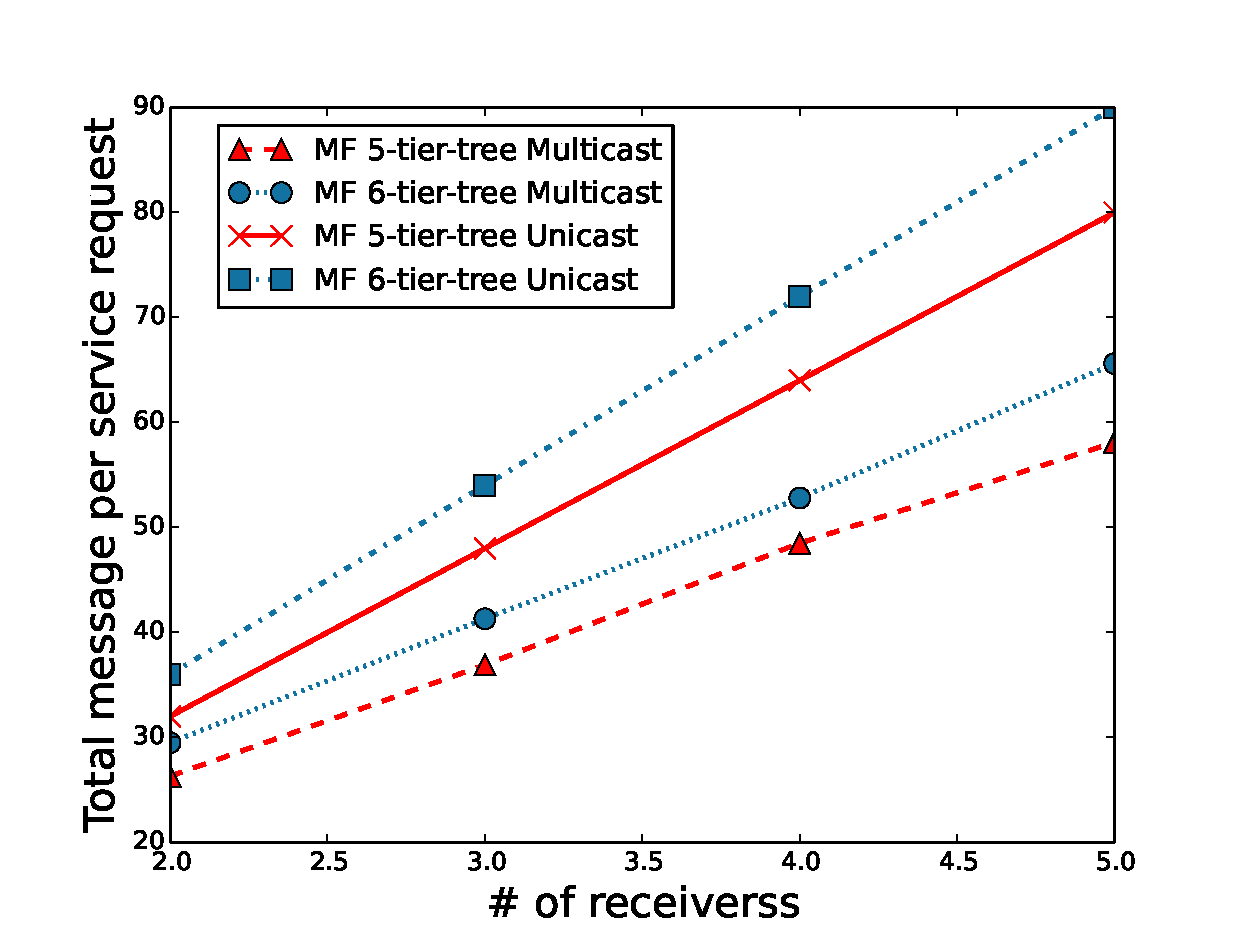
\includegraphics[width=\columnwidth]{figure/multicast_mf_overhead.eps}
\caption{\label{fig:mf_over}Overhead of service discovery}
\end{figure}
%\subsection{Service Discovery}
%\subsection{Multi-source Retrieval}

